Metode \textit{Synthetic Minority Over-sampling Technique} (SMOTE)
\cite{chawla2002smote} menggunakan pendekatan \textit{over-sampling} yang mana
kelas minoritas ditambah dengan membuat sampel sintetis, bukan dengan
mengganti sampel dari kelas mayoritas menjadi kelas minoritas.
Sampel sintetis dibuat lewat aplikasi dengan beroperasi pada
ruang fitur.
Kelas minoritas ditambah dengan mengambil setiap sampel-sampel dari kelas
minoritas dan membuat sampel sintetis di antara segmen garis yang menghubungkan
setiap tetangga terdekat (\textit{k-nearest-neighbors}, KNN) dari kelas
minoritas.
Instan dari KNN dipilih secara acak, bergantung dari jumlah
\textit{over-sampling} yang dibutuhkan.

\begin{figure}[htbp]
\centering
\setlength\fboxsep{4pt}
\fbox{
	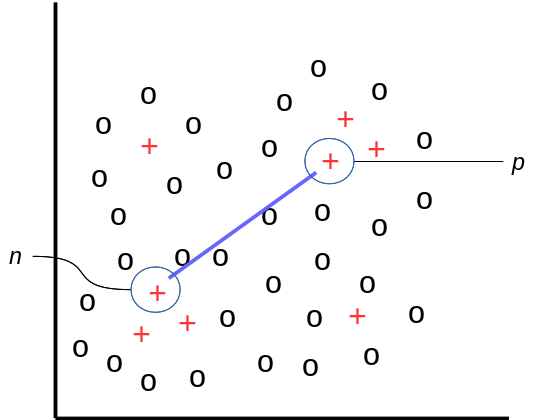
\includegraphics[keepaspectratio=true,scale=0.35]{SMOTE-example}
}
	\caption{
	Ilustrasi pembuatan sampel sintetis pada SMOTE.
	$p$ adalah sampel minoritas, $n$ adalah salah satu
	\textit{k-nearest-neighbors} dari $p$.
	Sampel sintetis yang baru akan berada digaris antara $p$ dan $n$.
	}
	\label{fig:smote}
\end{figure}

Sampel sintetis dibuat dengan cara berikut,
\begin{compactitem}%
	\item Hitung selisih antara vektor fitur (sampel) dengan tetangga
	terdekatnya.
	\item Kalikan selisih tersebut dengan angka ril acak antara 0 sampai 1,
	dan
	\item tambahkan hasilnya ke vektor fitur.
\end{compactitem}

Cara ini membuat sampel secara acak pada segmen garis antara dua fitur yang
terpilih, seperti yang terlihat pada gambar \ref{fig:smote}.
Pendekatan ini secara efektif mendorong wilayah pembelajaran dari kelas
minoritas menjadi lebih besar tanpa menyebabkan \textit{overfitting}.
Untuk fungsi selengkapnya dari SMOTE bisa dilihat pada algoritma \ref{alg:smote}.

\begin{center}
	\captionof{algorithm}{SMOTE}
	\label{alg:smote}
	\begin{algorithmic}[1]
\Require \\
$ P $: dataset minoritas \\
$ o $: persentase jumlah sampel sintetis yang akan dibuat \\
$ k $: jumlah tetangga terdekat dari sampel yang akan dibuat
\\
\Function{SMOTE}{$ P, o, k $}
	\State $ S \gets [] $
	\Comment Penampung untuk semua sampel sintetis yang akan dibuat.

	\State $ nsyn \gets 0 $
	\Comment Jumlah sampel sintetis yang akan dibuat.

	\State $ lenP \gets \Call{Length}{P} $

	\If{$o < 100$}
		\label{o_less_100}
		\State $ nsyn \gets (o / 100) \times lenP $
		\State $ P \gets \Call{RandomPickWithoutReplacement}{P, nsyn} $
	\Else
		\State $ nsyn \gets o / 100.0 $
	\EndIf

	\For{\textbf{each} $sample$ \textbf{in} $P$}
		\State $ neighbors \gets \Call{FindNeighbours}{P, sample, k} $
		\Comment Cari k buah tetangga terdekat dari $sample$ di P.

		\State $ s \gets \Call{CreateSynthetic}{sample, neighbors, nsyn} $

		\State $ \Call{S.Push}{s} $
	\EndFor

	\State \Return{S}
\EndFunction
\\
\Function{CreateSynthetic}{$ sample, neighbors, nsyn $}
	\State $ s \gets [] $
	\Comment Penampung untuk semua sampel sintetis yang akan dibuat.

	\State $ lenAttr \gets \Call{LengthAttribute}{sample} $
	\Comment Simpan jumlah atribut dari sampel.

	\For{$ x \gets 1,nsyn $}
		\State $ neighbor \gets \Call{RandomPick}{neighbors} $
		\State $ newsample \gets [] $
		\Comment Penampung untuk sampel sintetis yang baru.

		\For{$ y \gets 1,lenAttr $}
			\If{y \textbf{is} classAttribute}
				\State continue
			\EndIf

			\State $ nattr \gets neighbor.\Call{AttributeAt}{y} $
			\State $ sattr \gets sample.\Call{AttributeAt}{y} $
			\State $ diff \gets sattr - nattr $
			\State $ gap \gets \Call{Random}{0,1} $
			\State $ newAttr \gets nattr + (gap \times diff) $

			\State $ newsample.\Call{PushAttribute}{newAttr} $
		\EndFor

		\State $ \Call{s.Push}{newsample} $
	\EndFor

	\State \Return{s}
\EndFunction

	\end{algorithmic}
\end{center}

